\chapter{Conceptos Básicos}% \label{lbl-conceptos}
\section{Definición}% \label{lbl-definicion}
Una onda es una perturbación o fluctuación que se propaga a través de algún medio transportando energía. Se caracteriza por la porpagación de una perturbación a través de un medio.

La palabra `\textit{onda}' deriva de la palabra en latín `\textit{unda}', que significa ola, oleada o agua agitada.

Las ondas transfieren energía, no materia. En ciertas ocasiones, esa energía se puede interpretar como información significativa y se puede digitalizar.

\begin{grafica}
\centering
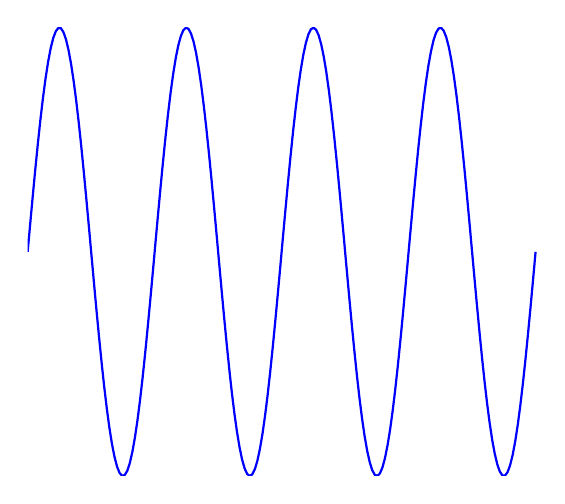
\begin{tikzpicture}
  \begin{axis}[
    xmin=0,xmax=8.5*pi,
    ymin=-1,ymax=1,
    axis lines = none,
    xtick={0},ytick={0}
    ]
    \addplot[color=blue,samples=200,domain=0:8*pi,thick]{sin(deg(x))};
  \end{axis}
\end{tikzpicture}
\caption{Onda simple}
\end{grafica}

\section{Elementos}
\begin{grafica}[H]
\centering
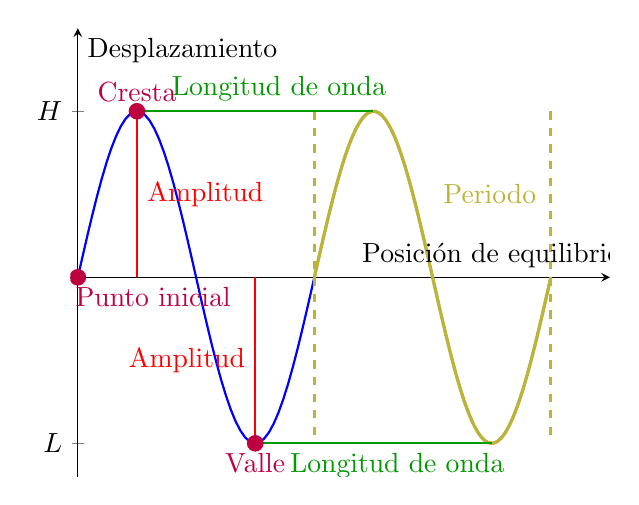
\begin{tikzpicture}
  \begin{axis}[
    xmin=-0.2,xmax=4.5*pi,
    ymin=-1.2,ymax=1.5,
    axis lines=middle,
    xtick={0},
    % xtick={pi/2,pi,3*pi/2,2*pi,5*pi/2,3*pi,7*pi/2,4*pi},
    % xticklabels={
    %   $\dfrac{\pi}{2}$,
    %   $\pi$,
    %   $\dfrac{3}{2}\pi$,
    %   $2\pi$,
    %   $\dfrac{5}{2}\pi$,
    %   $3\pi$,
    %   $\dfrac{7}{2}\pi$,
    %   $4\pi$
    % },
    ytick={-1,1},yticklabels={$L$,$H$},
    ylabel=Desplazamiento
    ]

    % Funcion senoidal
    \addplot[color=blue,samples=100,domain=0:4*pi,thick]{sin(deg(x))};

    % Punto inicial
    \fill[purple] (axis cs:0,0) circle[radius=3pt];
    \node[purple,below] at (axis cs:2,0) {Punto inicial};

    % Periodo
    \addplot[color=yellow!70!black,samples=100,domain=2*pi:4*pi,very thick]{sin(deg(x))};
    \node[yellow!70!black,right,very thick] at (axis cs:3*pi,0.5) {Periodo};
    \draw[yellow!70!black,dashed,very thick] (axis cs:2*pi,1) -- (axis cs:2*pi,-1);
    \draw[yellow!70!black,dashed,very thick] (axis cs:4*pi,1) -- (axis cs:4*pi,-1);

    % Amplitud
    \draw[red,thick] (axis cs:pi/2,0) -- (axis cs:pi/2,1) node[pos=0.5,right] {Amplitud};
    \draw[red,thick] (axis cs:3*pi/2,0) -- (axis cs:3*pi/2,-1) node[pos=0.5,left] {Amplitud};

    % Longitud de onda
    \draw[green!60!black,thick] (axis cs:pi/2,1) -- (axis cs:5*pi/2,1) node[pos=0.6,above] {Longitud de onda};
    \draw[green!60!black,thick] (axis cs:3*pi/2,-1) -- (axis cs:7*pi/2,-1) node[pos=0.6,below] {Longitud de onda};

    % Cresta
    \fill[purple] (axis cs:pi/2,1) circle[radius=3pt];
    \node[purple,above] at (axis cs:pi/2,1) {Cresta};

    % Valle
    \fill[purple] (axis cs:3*pi/2,-1) circle[radius=3pt];
    \node[purple,below] at (axis cs:3*pi/2,-1) {Valle};

    % Posicion de equilibrio
    \node[above] at (axis cs:7*pi/2,0) {Posición de equilibrio};
  \end{axis}
\end{tikzpicture}
\caption{Elementos de una onda}
\end{grafica}

\subsection{Posición de Equilibrio}
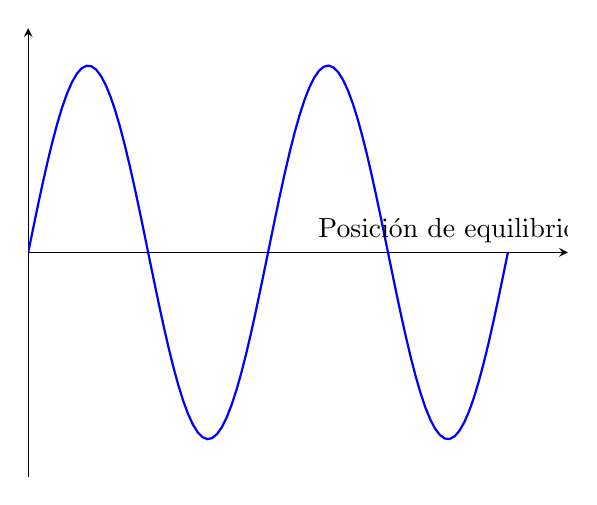
\begin{tikzpicture}
  \begin{axis}[
    xmin=0,xmax=4.5*pi,
    ymin=-1.2,ymax=1.2,
    axis lines=middle,
    xtick={0},
    ytick={0}
    ]

    % Funcion senoidal
    \addplot[color=blue,samples=100,domain=0:4*pi,thick]{sin(deg(x))};

    % Posicion de equilibrio
    \node[above] at (axis cs:7*pi/2,0) {Posición de equilibrio};
  \end{axis}
\end{tikzpicture}

\subsection{Desplazamiento}
Que tan lejos de la posición de equilibrio la onda oscila. Es la medida de cuánto se mueve una partícula en un medio de su estado de reposo cuando una onda pasa a través de ella.

Cuando una onda viaja a través de un medio, las partículas de ese medio vibran o se desplazan de su posición de equilibrio.

Se identifica con el eje de las ordenadas $y$ en un plano cartesiano.

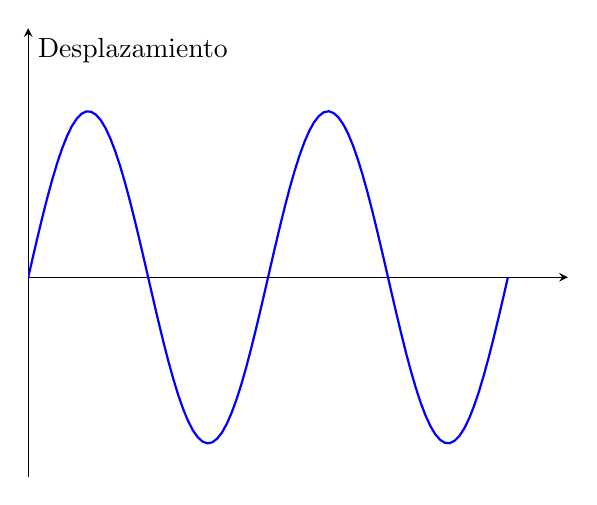
\begin{tikzpicture}
  \begin{axis}[
    xmin=0,xmax=4.5*pi,
    ymin=-1.2,ymax=1.5,
    axis lines=middle,
    xtick={0},
    ytick={0},
    ylabel=Desplazamiento
    ]

    % Funcion senoidal
    \addplot[color=blue,samples=100,domain=0:4*pi,thick]{sin(deg(x))};
  \end{axis}
\end{tikzpicture}

\subsection{Punto Inicial}
Este punto representa la posición inicial de la onda en el tiempo y el espacio, y se utiliza para definir la forma y el desplazamiento de la onda en cualquier instante posterior.

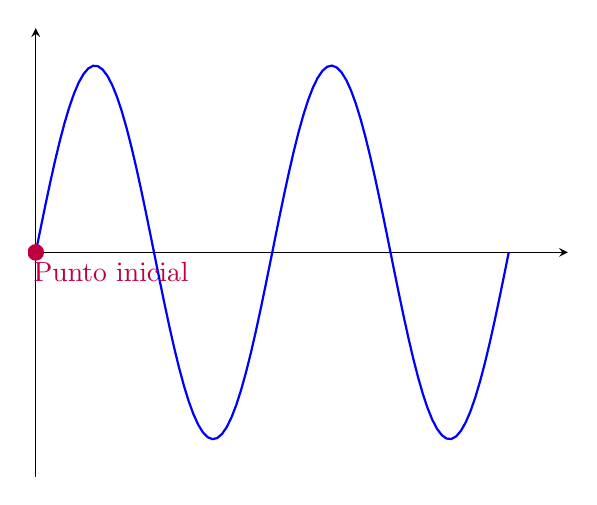
\begin{tikzpicture}
  \begin{axis}[
    xmin=-0.2,xmax=4.5*pi,
    ymin=-1.2,ymax=1.2,
    axis lines=middle,
    xtick={0},
    ytick={0}
    ]

    % Funcion senoidal
    \addplot[color=blue,samples=100,domain=0:4*pi,thick]{sin(deg(x))};

    % Punto inicial
    \fill[purple] (axis cs:0,0) circle[radius=3pt];
    \node[purple,below] at (axis cs:2,0) {Punto inicial};
  \end{axis}
\end{tikzpicture}

\subsection{Cresta}
Es un punto máximo que alcanza una onda al desplazarse. El punto más alto, donde la amplitud es máxima.

Es el punto más alejado de la posición de equilibrio en la dirección positiva del desplazamiento.

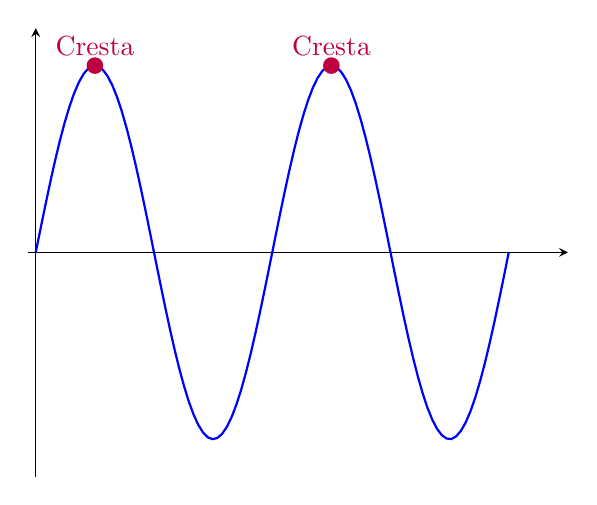
\begin{tikzpicture}
  \begin{axis}[
    xmin=-0.2,xmax=4.5*pi,
    ymin=-1.2,ymax=1.2,
    axis lines=middle,
    xtick={0},
    ytick={0}
    ]

    % Funcion senoidal
    \addplot[color=blue,samples=100,domain=0:4*pi,thick]{sin(deg(x))};

    % Cresta 1
    \fill[purple] (axis cs:pi/2,1) circle[radius=3pt];
    \node[purple,above] at (axis cs:pi/2,1) {Cresta};

    % Cresta 2
    \fill[purple] (axis cs:5*pi/2,1) circle[radius=3pt];
    \node[purple,above] at (axis cs:5*pi/2,1) {Cresta};
  \end{axis}
\end{tikzpicture}

\subsection{Valle}
Es un punto mínimo que alcanza una onda al desplazarse. El punto más bajo, donde la amplitud es mínima.

Es el punto más alejado de la posición de equilibrio en la dirección negativa del desplazamiento.

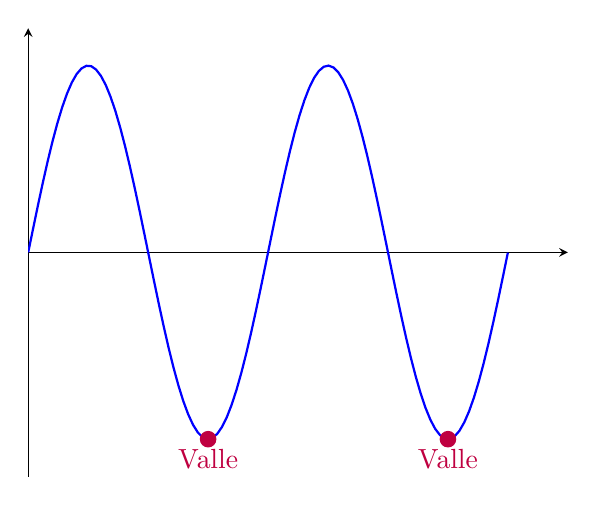
\begin{tikzpicture}
  \begin{axis}[
    xmin=0,xmax=4.5*pi,
    ymin=-1.2,ymax=1.2,
    axis lines=middle,
    xtick={0},
    ytick={0}
    ]

    % Funcion senoidal
    \addplot[color=blue,samples=100,domain=0:4*pi,thick]{sin(deg(x))};

    % Valle 1
    \fill[purple] (axis cs:3*pi/2,-1) circle[radius=3pt];
    \node[purple,below] at (axis cs:3*pi/2,-1) {Valle};

    % Valle 2
    \fill[purple] (axis cs:7*pi/2,-1) circle[radius=3pt];
    \node[purple,below] at (axis cs:7*pi/2,-1) {Valle};
  \end{axis}
\end{tikzpicture}

\subsection{Amplitud}
La amplitud es el desplazamiento máximo desde la posición de equilibrio. Se representa con la letra $A$.

La amplitud puede ser hacia arriba o hacia abajo con respecto a la posición de equilibrio.

En el eje de desplazamiento el límite superior se denomina $H$ y el inferior $L$.

{
\centering
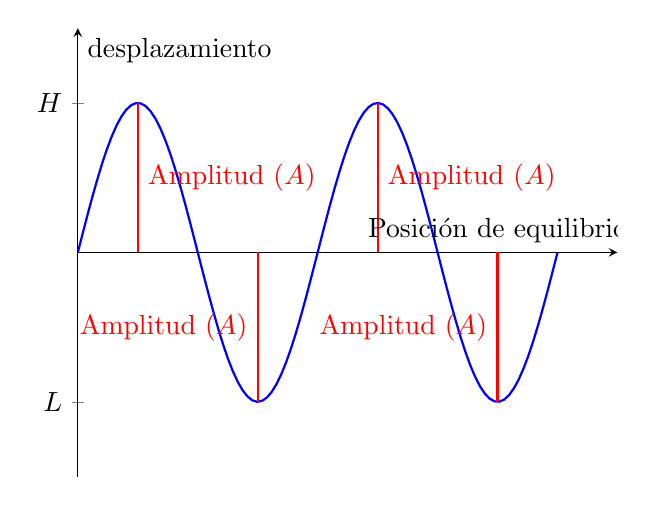
\begin{tikzpicture}
  \begin{axis}[
    xmin=-0,xmax=4.5*pi,
    ymin=-1.5,ymax=1.5,
    axis lines=middle,
    xtick={0},
    ytick={-1,1},yticklabels={$L$,$H$},
    ylabel = desplazamiento,
    ]

    % Funcion senoidal
    \addplot[color=blue,samples=100,domain=0:4*pi,thick]{sin(deg(x))};

    % Amplitud
    \draw[red,thick] (axis cs:pi/2,0) -- (axis cs:pi/2,1) node[pos=0.5,right] {Amplitud ($A$)};
    \draw[red,thick] (axis cs:3*pi/2,0) -- (axis cs:3*pi/2,-1) node[pos=0.5,left] {Amplitud ($A$)};
    \draw[red,thick] (axis cs:5*pi/2,0) -- (axis cs:5*pi/2,1) node[pos=0.5,right] {Amplitud ($A$)};
    \draw[red,thick] (axis cs:7*pi/2,0) -- (axis cs:7*pi/2,-1) node[pos=0.5,left] {Amplitud ($A$)};


    % Posicion de equilibrio
    \node[above] at (axis cs:7*pi/2,0) {Posición de equilibrio};

    % Label y
    % \node[right,rotate=90] at (axis cs:0,0) {desplazamiento};
  \end{axis}
\end{tikzpicture}
}

Para calcular la amplitud se puede hacer uso de los límites superior $(H)$ e inferior $(L)$ en el eje de desplazamiento $y$. Hay dos formas:

\subsubsection{Promedio de la resta de ambos límites}

Consiste en restar los límites y dividir entre dos.

\[
  A=\dfrac{H-L}{2}
\]

Adicionalmente se puede determinar el punto central. Hay dos formas:

Con respecto al límite superior $H$:

\[
  \text{punto central}=H-A
\]

Con respecto al límite inferiro $L$:

\[
  \text{punto central}=L+A
\]

\subsubsection{Promedio de la suma de ambos límites}

Consiste en obtener el promedio de los límites y determinar la diferencia entre los límites y el promedio.

\[
  \text{punto central} = \dfrac{H+L}{2}
\]

Luego se realiza una diferencia para hallar la amplitud $A$. Hay dos formas:

Con respecto al límite superior $H$:

\[
  A = H - \text{punto central}
\]

Con respecto al límite inferior $L$:

\[
  A = \text{punto central} - L
\]

\subsection{Distancia}
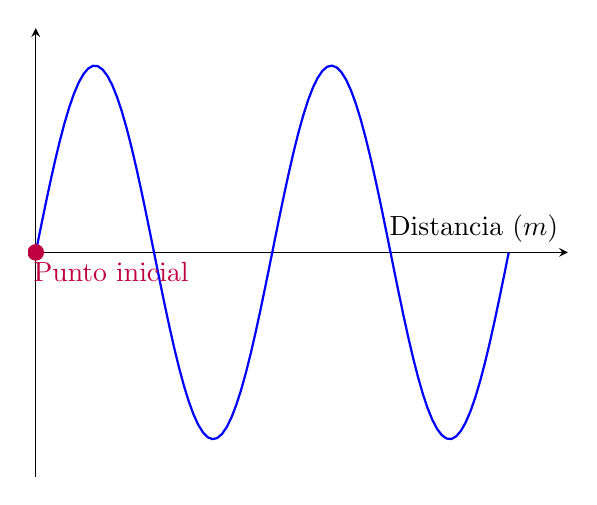
\begin{tikzpicture}
  \begin{axis}[
    xmin=-0.2,xmax=4.5*pi,
    ymin=-1.2,ymax=1.2,
    axis lines=middle,
    xtick={0},
    ytick={0},
    xlabel=Distancia ($m$)
    ]

    % Funcion senoidal
    \addplot[color=blue,samples=100,domain=0:4*pi,thick]{sin(deg(x))};

    % Punto inicial
    \fill[purple] (axis cs:0,0) circle[radius=3pt];
    \node[purple,below] at (axis cs:2,0) {Punto inicial};
  \end{axis}
\end{tikzpicture}

\subsection{Longitud de Onda}
Distancia entre dos puntos equivalentes consecutivos en un onda. Puede ser entre crestas, valles o puntos de corte con la posición de equiilibrio. Se representa con la letra griega lambda $\lambda$.

Es la distancia de una oscilación completa.

Se mide en unidades de longitud. El Sistema internacional utiliza metros $m$.

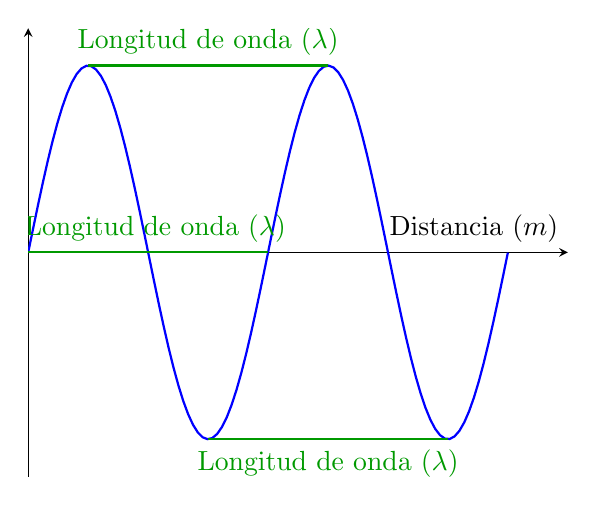
\begin{tikzpicture}
  \begin{axis}[
    xmin=0,xmax=4.5*pi,
    ymin=-1.2,ymax=1.2,
    axis lines=middle,
    xtick={0},
    ytick={0},
    xlabel=Distancia ($m$)
    ]

    % Funcion senoidal
    \addplot[color=blue,samples=100,domain=0:4*pi,thick]{sin(deg(x))};

    % Longitud de onda
    \draw[green!60!black,thick] (axis cs:0,0) -- (axis cs:2*pi,0) node[pos=0.53,above] {Longitud de onda ($\lambda$)};
    \draw[green!60!black,thick] (axis cs:pi/2,1) -- (axis cs:5*pi/2,1) node[pos=0.5,above] {Longitud de onda ($\lambda$)};
    \draw[green!60!black,thick] (axis cs:3*pi/2,-1) -- (axis cs:7*pi/2,-1) node[pos=0.5,below] {Longitud de onda ($\lambda$)};
  \end{axis}
\end{tikzpicture}

Considerando la distancia en metros y el número de ciclos u oscilaciones, se puede calcular de la siguiente manera:

\[\boxed{
  \lambda = \dfrac{\text{distancia} (m)}{\text{número de ciclos}}
}\]

\subsection{Tiempo}
Medida de la duración de la onda. Se representa mediante el eje de las abscisas $x$ en un plano cartesiano.

El Sistema Internacional utiliza el segundo $s$ como medida básica de tiempo.

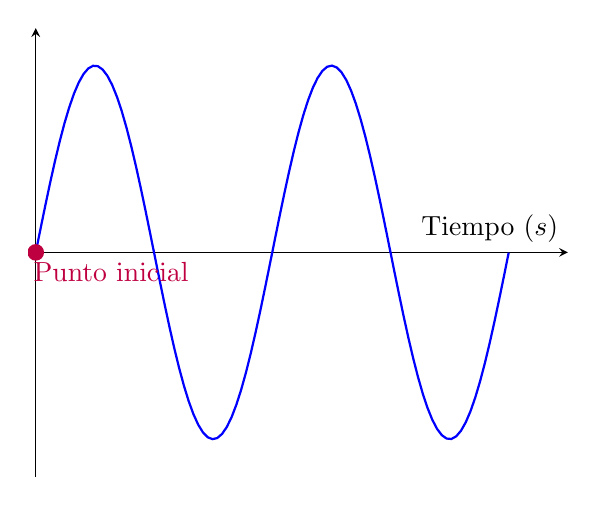
\begin{tikzpicture}
  \begin{axis}[
    xmin=-0.2,xmax=4.5*pi,
    ymin=-1.2,ymax=1.2,
    axis lines=middle,
    xtick={0},
    ytick={0},
    xlabel=Tiempo ($s$)
    ]

    % Funcion senoidal
    \addplot[color=blue,samples=100,domain=0:4*pi,thick]{sin(deg(x))};

    % Punto inicial
    \fill[purple] (axis cs:0,0) circle[radius=3pt];
    \node[purple,below] at (axis cs:2,0) {Punto inicial};
  \end{axis}
\end{tikzpicture}

\subsection{Periodo}
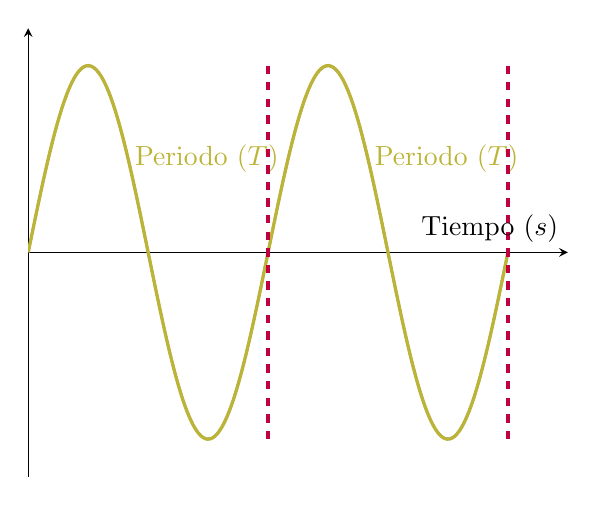
\begin{tikzpicture}
  \begin{axis}[
    xmin=0,xmax=4.5*pi,
    ymin=-1.2,ymax=1.2,
    axis lines=middle,
    xtick={0},
    ytick={0},
    xlabel=Tiempo ($s$)
    ]

    % Funcion senoidal
    \addplot[color=blue,samples=100,domain=0:4*pi,thick]{sin(deg(x))};

    % Periodo 1
    \addplot[color=yellow!70!black,samples=100,domain=2*pi:4*pi,very thick]{sin(deg(x))};
    \node[yellow!70!black,right,very thick] at (axis cs:2.8*pi,0.5) {Periodo ($T$)};

    % Periodo 2
    \addplot[color=yellow!70!black,samples=100,domain=0:2*pi,very thick]{sin(deg(x))};
    \node[yellow!70!black,right,very thick] at (axis cs:0.8*pi,0.5) {Periodo ($T$)};

    % Lineas verticales
    \draw[purple,dashed,very thick] (axis cs:2*pi,1) -- (axis cs:2*pi,-1);
    \draw[purple,dashed,very thick] (axis cs:4*pi,1) -- (axis cs:4*pi,-1);
  \end{axis}
\end{tikzpicture}

\subsection{Frecuencia}
Número de ciclos completos que la onda realiza en un segundo. Se representa con la letra $f$ minúscula. Se mide en Hertz $Hz$.

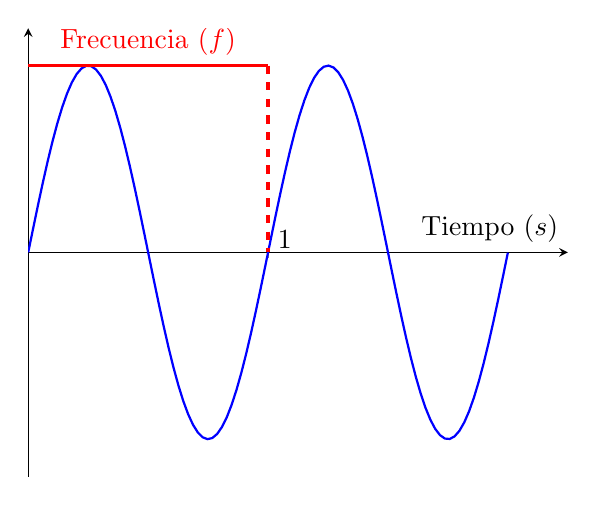
\begin{tikzpicture}
  \begin{axis}[
    xmin=0,xmax=4.5*pi,
    ymin=-1.2,ymax=1.2,
    axis lines=middle,
    xtick={0},
    xtick={2*pi},xticklabels={1},
    xticklabel style={anchor=south west},
    ytick={0},
    xlabel=Tiempo ($s$)
    ]

    % Funcion senoidal
    \addplot[color=blue,samples=100,domain=0:4*pi,thick]{sin(deg(x))};

    % Frecuencia
    \draw[red,thick] (axis cs:0,1) -- (axis cs:2*pi,1) node[pos=0.5,above] {Frecuencia ($f$)};

    % Linea vertical
    \draw[red,dashed,very thick] (axis cs:2*pi,1) -- (axis cs:2*pi,0);
  \end{axis}
\end{tikzpicture}

La frecuencia es el inverso del periodo.

\begin{listequbox}
  {f = \dfrac{1}{T}}{equfrecuencia}{Relación entre frecuencia y periodo}
\end{listequbox}

Interpretando la ecuación \ref{equfrecuencia} en sentido contrario, el periodo es el inverso de la frecuencia.

\[\boxed{
  T = \dfrac{1}{f}
}\]

Teniendo en cuenta el número de ciclos y el periodo en segundos, se puede definir la frecuencia como la cantidad de ciclos por segundo

Considerando esta relación, la unidad de medida de la frecuencia es $\dfrac{1}{s}$ o $s^{-1}$. Esto equivale a un Hertz $Hz$.

\[\boxed{
  \dfrac{1}{s}=s^{-1}=Hz
}\]

